\subsection{Αποτελέσματα}

\subsubsection{Δημογραφικά}

Οι συμμετέχοντες στη μελέτη και αξιολόγηση του παιχνιδιού ανήκαν κυρίως στην ηλικιακή ομάδα των 19-31 ετών(εικόνα \ref{fig:age}), με τον αριθμό των αρσενικών στο 54.8 \% και των θηλυκών στο 45.2 \%(εικόνα \ref{fig:gender}). Αυτή η ηλικιακή ομάδα είναι ιδιαίτερα σημαντική για την ανάπτυξη και την αξιολόγηση εκπαιδευτικών παιχνιδιών, ειδικά σε θέματα που αφορούν την εκμάθηση αλγορίθμων και προγραμματισμού.

Σε αυτές τις ηλικίες, οι νέοι συχνά σπουδάζουν σε πανεπιστήμια ή τεχνολογικά ιδρύματα, όπου διδάσκονται προγραμματισμό και αλγορίθμους. Το ενδιαφέρον για αυτούς τους τομείς συνήθως ενισχύεται μέσω των ακαδημαϊκών τους σπουδών και των εργαστηρίων που παρακολουθούν.

Η ηλικιακή ομάδα 19-31 ετών είναι επίσης εκείνη που υιοθετεί εύκολα νέες τεχνολογίες και είναι εξοικειωμένη με ψηφιακές πλατφόρμες, γεγονός που τους καθιστά κατάλληλους για τη δοκιμή και αξιολόγηση εκπαιδευτικών εργαλείων. Έχουν την ικανότητα να παρέχουν ουσιαστική ανατροφοδότηση για τη χρηστικότητα και την αποτελεσματικότητα του παιχνιδιού, βοηθώντας στη βελτίωσή του.

Η ισορροπία μεταξύ αρσενικών και θηλυκών συμμετεχόντων εξασφαλίζει ότι λαμβάνονται υπόψη ποικίλες απόψεις και εμπειρίες, καθιστώντας το παιχνίδι πιο προσιτό και ελκυστικό για όλους τους χρήστες.

\begin{figure}[H]
    \centering
    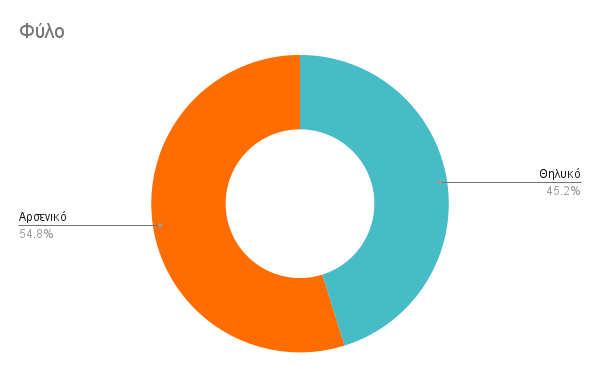
\includegraphics[width=0.7\linewidth]{sections/5/2/images/gender}
    \caption{Κατανομή συμμετεχόντων ανά φύλο}
    \label{fig:gender}
\end{figure}

\begin{figure}[H]
    \centering
    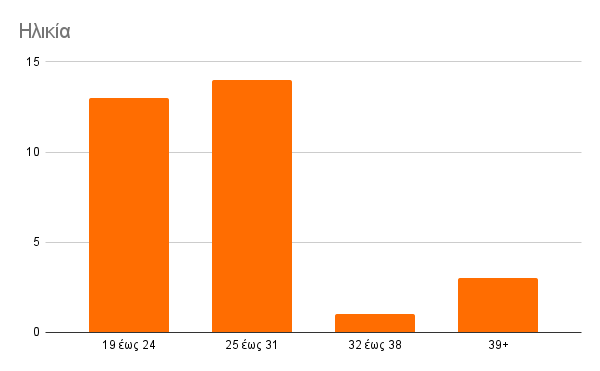
\includegraphics[width=0.7\linewidth]{sections/5/2/images/age}
    \caption{Κατανομή συμμετεχόντων ανά ηλικιακή ομάδα}
    \label{fig:age}
\end{figure}

% ========================================

\subsubsection{Προϋπάρχουσες γνώσεις}

Στους συμμετέχοντες παρατηρείται μια ισορροπία στις προηγούμενες γνώσεις όσον αφορά τους αλγόριθμους και τα παιχνίδια, με τα άτομα που είχαν προηγούμενη εμπειρία από αλγόριθμους στο 51.6 \%(εικόνα \ref{fig:do_you_have_previous_experience_of_algorithms}) και τα άτομα που είχαν προηγούμενη εμπειρία από παιχνίδια στο 58.1 \%(εικόνα \ref{fig:do_you_have_previous_gaming_experience}). Από εκείνους που είχαν εμπειρία με αλγόριθμους, η πλειοψηφία απέκτησε τις γνώσεις της μέσω ακαδημαϊκών σπουδών. Αντίθετα, από εκείνους με εμπειρία στα παιχνίδια, η συντριπτική πλειοψηφία απέκτησε τις γνώσεις της μέσω video games.

Αυτή η διαφοροποίηση στις πηγές γνώσης είναι σημαντική, καθώς δείχνει ότι οι συμμετέχοντες έχουν διαφορετικά υπόβαθρα και εμπειρίες που επηρεάζουν την αλληλεπίδρασή τους με το παιχνίδι. Οι ακαδημαϊκές γνώσεις στους αλγόριθμους παρέχουν μια θεωρητική και συστηματική βάση, ενώ η εμπειρία από τα video games δίνει έμφαση στη διαδραστικότητα και την πρακτική εφαρμογή. Η συνύπαρξη αυτών των δύο τύπων γνώσεων στους συμμετέχοντες συμβάλλει στην πληρέστερη αξιολόγηση του παιχνιδιού από διαφορετικές οπτικές γωνίες.

\begin{figure}[H]
    \centering
    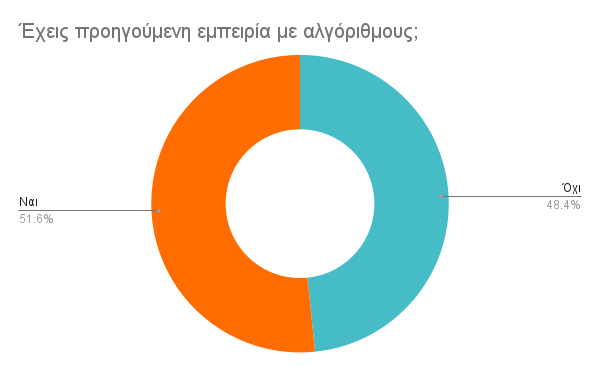
\includegraphics[width=0.7\linewidth]{sections/5/2/images/do_you_have_previous_experience_of_algorithms}
    \caption{Κατανομή συμμετεχόντων με βάση την προϋπάρχουσα εμπειρία αλγορίθμων}
    \label{fig:do_you_have_previous_experience_of_algorithms}
\end{figure}

\begin{figure}[H]
    \centering
    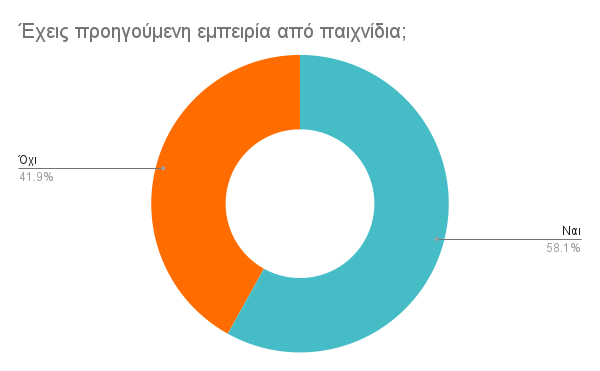
\includegraphics[width=0.7\linewidth]{sections/5/2/images/do_you_have_previous_gaming_experience}
    \caption{Κατανομή συμμετεχόντων με βάση την προϋπάρχουσα εμπειρία παιχνιδιών}
    \label{fig:do_you_have_previous_gaming_experience}
\end{figure}

% ========================================

\subsubsection{Αλγόριθμοι}

Η πλειοψηφία των συμμετεχόντων επέλεξε να χρησιμοποιήσει και τους δύο αλγόριθμους που υπήρχαν στο παιχνίδι. Οι υπόλοιποι προτίμησαν τον αλγόριθμο Bubble Sort, πιθανώς επειδή είναι η πρώτη επιλογή στη λίστα του παιχνιδιού(εικόνα \ref{fig:what_algorithm_did_you_use}).

Δεν έχει ελεγχθεί η υπόθεση αυτή, όμως καταγράφεται ως παρατήρηση ότι η προτίμηση πιθανόν να υποδηλώνει ότι η τοποθέτηση των επιλογών μπορεί να επηρεάσει τις αποφάσεις των χρηστών. Η χρήση και των δύο αλγορίθμων από το 61.3 \% των συμμετεχόντων δείχνει επίσης ενδιαφέρον για την εξερεύνηση και κατανόηση των διαφορετικών μεθόδων που προσφέρει το παιχνίδι. Η τάση αυτή είναι σημαντική για τους σχεδιαστές εκπαιδευτικών παιχνιδιών, καθώς δείχνει ότι η διάταξη και η παρουσίαση των επιλογών μπορεί να καθοδηγήσει τη συμπεριφορά των χρηστών και να ενθαρρύνει τη μάθηση.

\begin{figure}[H]
    \centering
    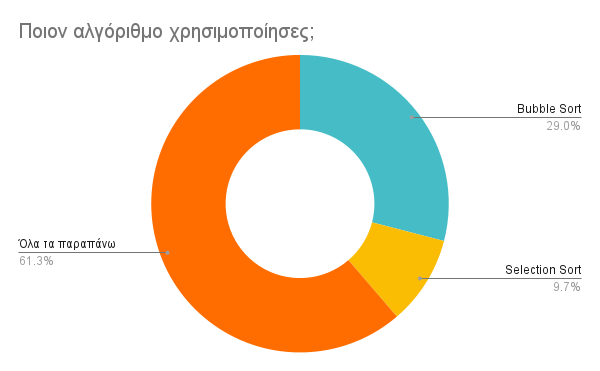
\includegraphics[width=0.7\linewidth]{sections/5/2/images/what_algorithm_did_you_use}
    \caption{Οι αλγόριθμοι που χρησιμοποίησαν οι συμμετέχοντες}
    \label{fig:what_algorithm_did_you_use}
\end{figure}

\textbf{Bubble Sort}

Φαίνεται ότι αρκετοί από τους συμμετέχοντες είχαν γνώση του Bubble Sort, ενώ άλλοι δεν είχαν(εικόνα \ref{fig:did_you_know_the_functionality_of_bubblesort}), κάτι που συνάδει με τα ποσοστά αυτών που είχαν προηγούμενη εμπειρία με αλγόριθμους. Αυτή η διαφοροποίηση δείχνει ότι ορισμένοι συμμετέχοντες είχαν ήδη εξοικείωση με τους βασικούς αλγορίθμους ταξινόμησης μέσω των σπουδών τους ή άλλων εμπειριών, ενώ άλλοι μάθαιναν για πρώτη φορά κατά τη διάρκεια του παιχνιδιού.

\begin{figure}[H]
    \centering
    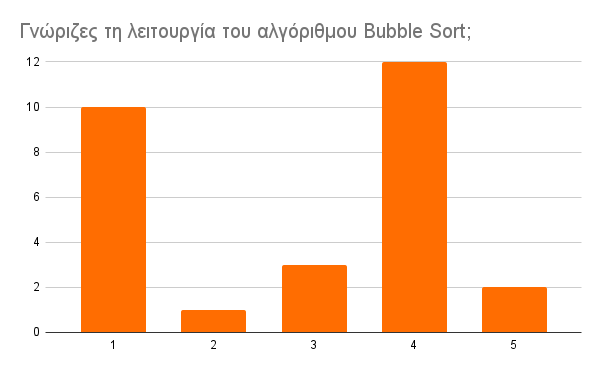
\includegraphics[width=0.7\linewidth]{sections/5/2/images/did_you_know_the_functionality_of_bubblesort}
    \caption{Κατανομή συμμετεχόντων με βάση τη γνώση του αλγορίθμου Bubble Sort}
    \label{fig:did_you_know_the_functionality_of_bubblesort}
\end{figure}

Η πλειοψηφία έπαιξε το επίπεδο δυσκολίας Guided 1 έως 3 φορές(εικόνα \ref{fig:bubblesort_guided_usages}), υποδεικνύοντας ότι για τους περισσότερους συμμετέχοντες, αυτές οι προσπάθειες ήταν αρκετές για να κατανοήσουν τη λειτουργία του αλγορίθμου και να προχωρήσουν στο επόμενο επίπεδο δυσκολίας. Το Guided επίπεδο φαίνεται να παρέχει επαρκή καθοδήγηση ώστε οι παίκτες να αισθάνονται άνετοι με τις βασικές αρχές του αλγορίθμου σε σύντομο χρονικό διάστημα.

\begin{figure}[H]
    \centering
    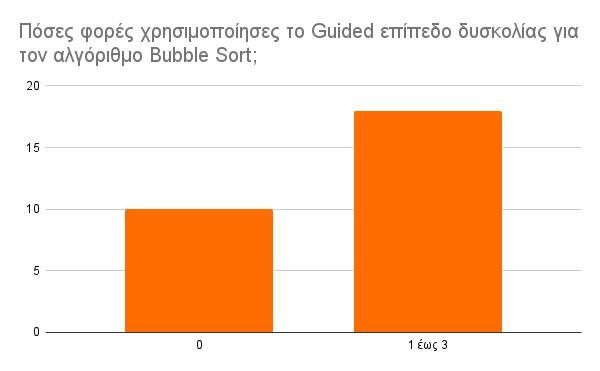
\includegraphics[width=0.7\linewidth]{sections/5/2/images/bubblesort_guided_usages}
    \caption{Αριθμός φορών που έπαιξαν το επίπεδο Guided για τον αλγόριθμο Bubble Sort}
    \label{fig:bubblesort_guided_usages}
\end{figure}

Παράλληλα, αρκετοί συμμετέχοντες επέλεξαν να παραλείψουν εντελώς το επίπεδο Guided(εικόνα \ref{fig:bubblesort_guided_usages}) και πήγαν κατευθείαν στο επίπεδο Time Trial(εικόνα \ref{fig:bubblesort_timetrial_usages}). Αυτό μπορεί να υποδεικνύει είτε αυτοπεποίθηση στις γνώσεις τους είτε προτίμηση για μια πιο άμεση πρόκληση. Οι παίκτες που ήταν εξοικειωμένοι με τους αλγόριθμους μπορεί να θεώρησαν περιττό το Guided επίπεδο και να προτίμησαν να δοκιμάσουν τις δεξιότητές τους σε πραγματικές συνθήκες χρονικής πίεσης.

\begin{figure}[H]
    \centering
    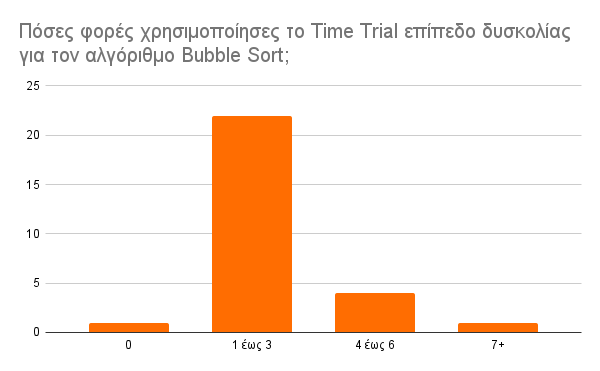
\includegraphics[width=0.7\linewidth]{sections/5/2/images/bubblesort_timetrial_usages}
    \caption{Αριθμός φορών που έπαιξαν το επίπεδο Time Trial για τον αλγόριθμο Bubble Sort}
    \label{fig:bubblesort_timetrial_usages}
\end{figure}

Είναι επίσης αξιοσημείωτο ότι όσοι έπαιξαν το επίπεδο δυσκολίας Time Trial περισσότερες από 3 φορές, το έκαναν είτε επειδή έχαναν συνεχώς είτε επειδή προσπαθούσαν να πετύχουν τον καλύτερο χρόνο από όλους τους παίκτες. Αυτό δείχνει δύο κύριες τάσεις: από τη μία, υπάρχουν παίκτες που χρησιμοποιούν τις επιπλέον προσπάθειες για να βελτιώσουν τις δεξιότητές τους και να ξεπεράσουν τις δυσκολίες που αντιμετωπίζουν, και από την άλλη, υπάρχουν εκείνοι με ανταγωνιστικό πνεύμα που επιδιώκουν να επιτύχουν κορυφαίες επιδόσεις και να συγκρίνουν τα αποτελέσματά τους με άλλους παίκτες.

Αυτές οι παρατηρήσεις υπογραμμίζουν τη σημασία της ύπαρξης διαφόρων επιπέδων δυσκολίας και τύπων προκλήσεων σε εκπαιδευτικά παιχνίδια. Παρέχοντας καθοδήγηση για τους αρχάριους και ανταγωνιστικές προκλήσεις για τους πιο προχωρημένους, το παιχνίδι μπορεί να καλύψει τις ανάγκες και τα ενδιαφέροντα ενός ευρέος φάσματος χρηστών, καθιστώντας την εκπαιδευτική εμπειρία πιο ελκυστική και αποτελεσματική για όλους.

\textbf{Selection Sort}

Τα αποτελέσματα για τον αλγόριθμο Selection Sort γενικά συνάδουν με αυτά του Bubble Sort, με την ιδιαιτερότητα ότι δεν υπάρχουν άτομα που έπαιξαν περισσότερες από 3 φορές το επίπεδο Time Trial(εικόνα \ref{fig:selectionsort_timetrial_usages}). Αυτό πιθανόν συμβαίνει επειδή ο αλγόριθμος Selection Sort είναι αρκετά πιο γρήγορος και ευκολότερος στην εκτέλεση από ανθρώπους, μειώνοντας την πιθανότητα λαθών και καθιστώντας ευκολότερη την επίτευξη γρήγορων χρόνων.

\begin{figure}[H]
    \centering
    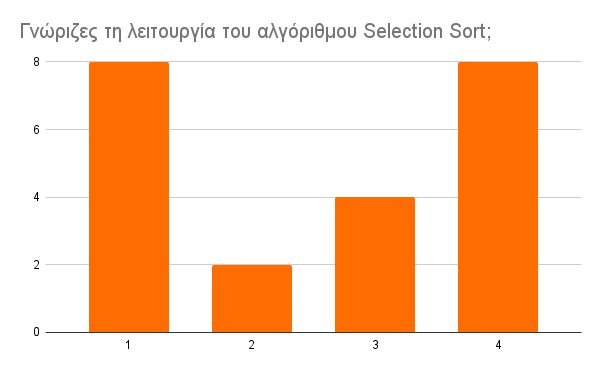
\includegraphics[width=0.7\linewidth]{sections/5/2/images/did_you_know_the_functionality_of_selectionsort}
    \caption{Κατανομή συμμετεχόντων με βάση τη γνώση του αλγορίθμου Selection Sort}
    \label{fig:did_you_know_the_functionality_of_selectionsort}
\end{figure}

\begin{figure}[H]
    \centering
    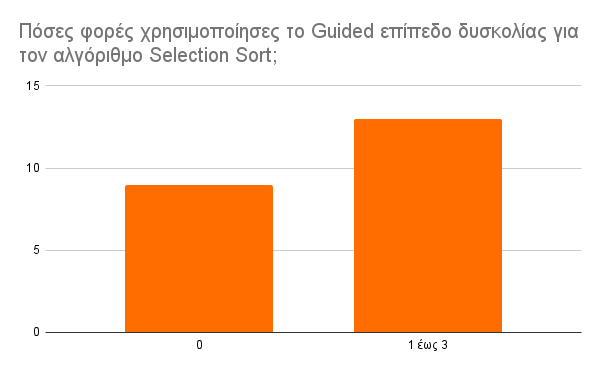
\includegraphics[width=0.7\linewidth]{sections/5/2/images/selectionsort_guided_usages}
    \caption{Αριθμός φορών που έπαιξαν το επίπεδο Guided για τον αλγόριθμο Selection Sort}
    \label{fig:selectionsort_guided_usages}
\end{figure}

\begin{figure}[H]
    \centering
    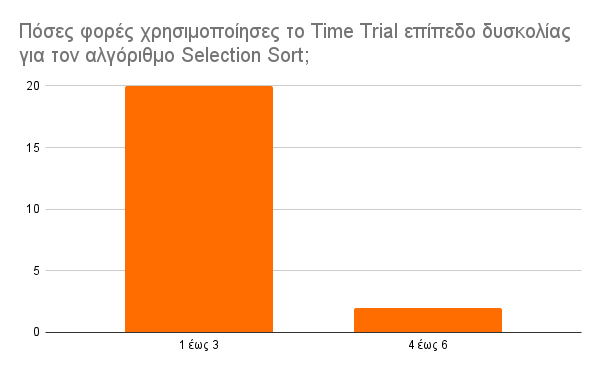
\includegraphics[width=0.7\linewidth]{sections/5/2/images/selectionsort_timetrial_usages}
    \caption{Αριθμός φορών που έπαιξαν το επίπεδο Time Trial για τον αλγόριθμο Selection Sort}
    \label{fig:selectionsort_timetrial_usages}
\end{figure}

Η απουσία συμμετεχόντων που έπαιξαν περισσότερες από 3 φορές το επίπεδο Time Trial υποδηλώνει ότι οι περισσότεροι χρήστες κατάφεραν να επιτύχουν ικανοποιητικά αποτελέσματα σε λιγότερες προσπάθειες. Ο Selection Sort, ως αλγόριθμος, είναι πιο απλός και αποτελεσματικός για τους ανθρώπους, καθώς απαιτεί λιγότερες ανταλλαγές και είναι πιο εύκολο να παρακολουθηθεί και να εφαρμοστεί.

Αυτή η παρατήρηση δείχνει ότι οι συμμετέχοντες μπορούσαν να κατανοήσουν και να εφαρμόσουν τον αλγόριθμο Selection Sort πιο γρήγορα και αποτελεσματικά σε σχέση με τον Bubble Sort. Το γεγονός ότι οι χρήστες πέτυχαν γρήγορους χρόνους και λιγότερα λάθη σε λιγότερες προσπάθειες υποδηλώνει ότι ο αλγόριθμος αυτός είναι πιο προσιτός και κατανοητός για εκπαιδευτικούς σκοπούς.

Συνολικά, η σύγκριση των δύο αλγορίθμων δείχνει ότι, ενώ και οι δύο μπορούν να διδαχθούν μέσω του παιχνιδιού, ο Selection Sort προσφέρει μια πιο εύκολη και άμεση εμπειρία μάθησης. Αυτό είναι σημαντικό για τους σχεδιαστές εκπαιδευτικών εργαλείων, καθώς επισημαίνει την ανάγκη για την ενσωμάτωση αλγορίθμων που είναι εύκολοι να κατανοηθούν και να εφαρμοστούν, ώστε να ενισχυθεί η μάθηση και η αυτοπεποίθηση των χρηστών.

% ========================================

\subsubsection{\acrshort{sus}}

Το σκορ \acrshort{sus} υπολογίζεται ως εξής: για τις θετικές ερωτήσεις (1, 3, 5, 7, 9), αφαιρείται το 1 από τη βαθμολογία τους, ενώ για τις αρνητικές ερωτήσεις (2, 4, 6, 8, 10), η βαθμολογία αφαιρείται από το 5. Το τελικό σκορ κυμαίνεται από 0 έως 100, με το 100 να υποδηλώνει άψογη χρηστικότητα και εξαιρετική εμπειρία χρήσης, ενώ σκορ κάτω από 50 υποδηλώνουν σοβαρή ανεπάρκεια στη χρηστικότητα και ανάγκη για ουσιαστικές βελτιώσεις.

Το μεγαλύτερο ποσοστό των απαντήσεων κυμαίνεται στο εύρος 60 έως 80, με το μέσο σκορ να είναι 75,72 \%(εικόνα \ref{fig:sus_score}), υποδηλώνοντας ότι οι χρήστες βρήκαν το παιχνίδι ευχάριστο και εύχρηστο.

\begin{figure}[H]
    \centering
    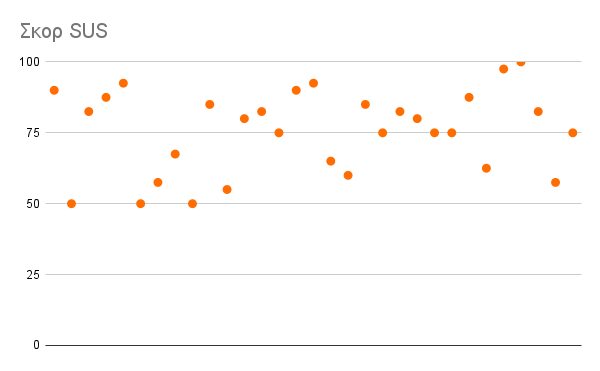
\includegraphics[width=0.7\linewidth]{sections/5/2/images/sus_score}
    \caption{Κατανομή σκορ \acrshort{sus}}
    \label{fig:sus_score}
\end{figure}

Αυτή η κατανομή των σκορ δείχνει ότι η πλειονότητα των χρηστών είχε μια θετική εμπειρία με το παιχνίδι, αναγνωρίζοντας την ευκολία στη χρήση και την ευχάριστη διάδραση. Το μέσο σκορ 75,72 \% τοποθετεί το παιχνίδι πάνω από τον μέσο όρο της χρηστικότητας, υποδεικνύοντας ότι οι περισσότερες πτυχές του είναι καλά σχεδιασμένες και λειτουργικές.

Τα αποτελέσματα αυτά είναι σημαντικά για τους σχεδιαστές του παιχνιδιού, καθώς επιβεβαιώνουν ότι η γενική χρηστικότητα είναι σε καλό επίπεδο, αλλά υποδεικνύουν και περιοχές όπου μπορεί να γίνει περαιτέρω βελτίωση. Η συνεχής ανατροφοδότηση από τους χρήστες και η προσαρμογή στις ανάγκες τους μπορούν να βοηθήσουν στη διατήρηση και την αύξηση αυτών των υψηλών ποσοστών ικανοποίησης, καθιστώντας το παιχνίδι ακόμα πιο αποτελεσματικό και ελκυστικό.

Τα δεδομένα αυτά τονίζουν τη σημασία της χρήσης του \acrshort{sus} ως εργαλείου αξιολόγησης της εμπειρίας χρήστη, επιτρέποντας μια σαφή και μετρήσιμη αξιολόγηση της χρηστικότητας του παιχνιδιού και καθοδηγώντας τις μελλοντικές βελτιώσεις.

% ========================================

\subsubsection{Εμπειρία χρηστών}

Η πλειοψηφία των συμμετεχόντων δήλωσε ότι βρήκε το παιχνίδι πολύ ενδιαφέρον και ότι θα έπαιζαν ξανά για να δοκιμάσουν διαφορετικούς αλγόριθμους. Όσοι δεν ήταν ικανοποιημένοι εξέφρασαν τη δυσαρέσκειά τους για την έλλειψη σαφών οδηγιών για κάθε αλγόριθμο. Ανέφεραν ότι θα ήθελαν έναν καλύτερο τρόπο για να κατανοήσουν τη λειτουργία των αλγορίθμων πριν ξεκινήσουν να παίζουν.

\begin{figure}[H]
    \centering
    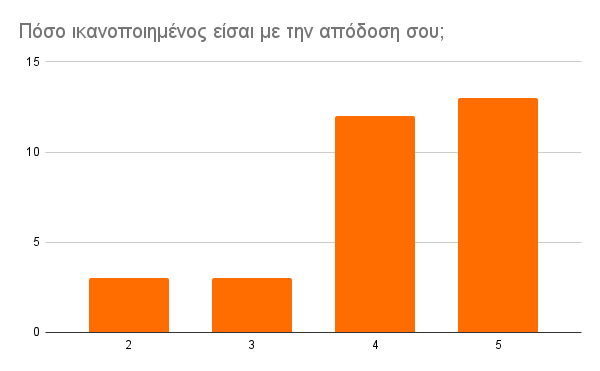
\includegraphics[width=0.7\linewidth]{sections/5/2/images/performance_satisfaction}
    \caption{Ικανοποίηση των συμμετεχόντων με την απόδοση τους}
    \label{fig:performance_satisfaction}
\end{figure}

\begin{figure}[H]
    \centering
    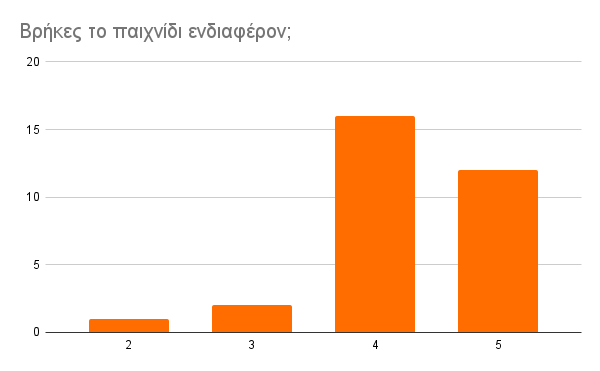
\includegraphics[width=0.7\linewidth]{sections/5/2/images/did_you_find_the_game_interesting}
    \caption{Ενδιαφέρον των συμμετεχόντων για το παιχνίδι}
    \label{fig:did_you_find_the_game_interesting}
\end{figure}

\begin{figure}[H]
    \centering
    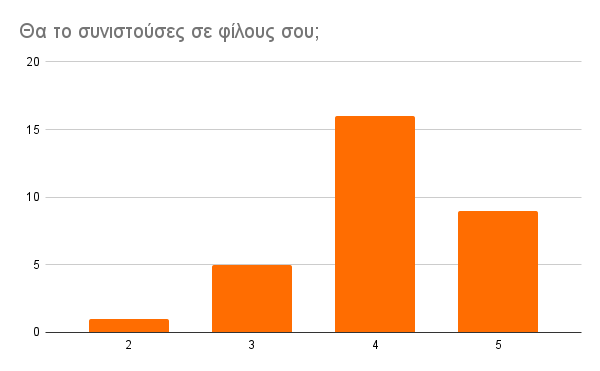
\includegraphics[width=0.7\linewidth]{sections/5/2/images/would_you_reccomend_it_to_your_friends}
    \caption{Αριθμός συμμετεχόντων που θα πρότειναν το παιχνίδι σε φίλους}
    \label{fig:would_you_reccomend_it_to_your_friends}
\end{figure}

\begin{figure}[H]
    \centering
    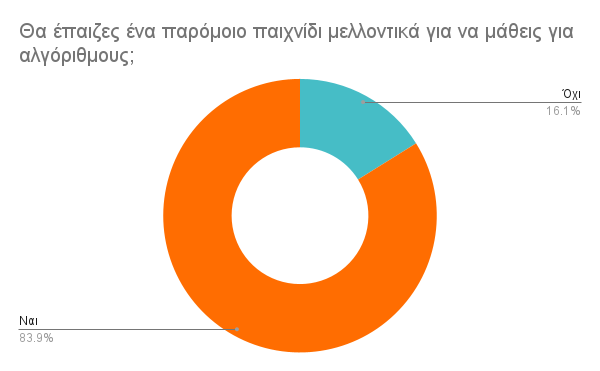
\includegraphics[width=0.7\linewidth]{sections/5/2/images/would_you_play_a_similar_game_in_the_future}
    \caption{Αριθμός συμμετεχόντων που θα έπαιζαν ξανά ένα παρόμοιο παιχνίδι}
    \label{fig:would_you_play_a_similar_game_in_the_future}
\end{figure}

Παρατηρήθηκε επίσης ότι στο Guided επίπεδο δυσκολίας οι παίκτες προσπαθούσαν αμέσως να αλληλεπιδράσουν με τα κλειδωμένα κουτιά, παρότι έγραφαν πάνω ότι ήταν κλειδωμένα, κάτι που μπορεί να υποδεικνύει πως το κίτρινο χρώμα τους τραβά την προσοχή.

Αυτές οι παρατηρήσεις παρέχουν πολύτιμη ανατροφοδότηση για τους σχεδιαστές του παιχνιδιού. Η γενική ικανοποίηση των συμμετεχόντων είναι ενθαρρυντική και υποδεικνύει ότι το παιχνίδι είναι ενδιαφέρον και διασκεδαστικό. Ωστόσο, οι ανησυχίες σχετικά με τις σαφείς οδηγίες και την κατανόηση των αλγορίθμων είναι σημαντικές για τη βελτίωση της εμπειρίας χρήστη.

Όσον αφορά την αλληλεπίδραση με τα κλειδωμένα κουτιά στο Guided επίπεδο, η χρήση του κίτρινου χρώματος φαίνεται να τραβά την προσοχή των παικτών, κάτι που μπορεί να προκαλεί σύγχυση. Μια πιθανή βελτίωση θα ήταν να αλλάξει το χρώμα ή να προστεθεί μια επιπλέον ένδειξη που να εξηγεί γιατί τα κουτιά είναι κλειδωμένα και πότε θα γίνουν προσβάσιμα. Αυτό θα μπορούσε να μειώσει την απογοήτευση και να διευκολύνει τη ροή του παιχνιδιού.

Συνολικά, η ανατροφοδότηση από τους συμμετέχοντες είναι εξαιρετικά πολύτιμη για τη συνεχή βελτίωση του παιχνιδιού. Καθώς οι σχεδιαστές λαμβάνουν υπόψη τις προτάσεις και τις παρατηρήσεις των χρηστών, μπορούν να κάνουν προσαρμογές που θα ενισχύσουν την εκπαιδευτική αξία και τη χρηστικότητα του παιχνιδιού, καθιστώντας το ακόμα πιο ελκυστικό και αποτελεσματικό για όλους τους παίκτες.

% ========================================

\subsubsection{Στατιστικά διαχειριστικού}

Στο διαχειριστικό σύστημα που έχουν πρόσβαση οι εκπαιδευτικοί, παρουσιάζονται βασικά δεδομένα για τους χρήστες και τη χρήση της πλατφόρμας(εικόνα \ref{fig:admin_dashboard_statistics_results}). Εδώ, μπορούν να δουν τους χρήστες που έχουν παίξει το παιχνίδι και τους αλγόριθμους που έχουν ολοκληρώσει. Παρατηρείται ότι περίπου το 50 \% των επιπέδων Time Trial είναι επιτυχή. Αυτό το ποσοστό επιτυχίας δείχνει ότι ενώ οι μισοί περίπου παίκτες καταφέρνουν να ολοκληρώσουν επιτυχώς τα επίπεδα, υπάρχει ακόμα ένα σημαντικό ποσοστό που αντιμετωπίζει δυσκολίες, υποδεικνύοντας την ανάγκη για περαιτέρω υποστήριξη ή προσαρμογές στο παιχνίδι.

\begin{figure}[H]
    \centering
    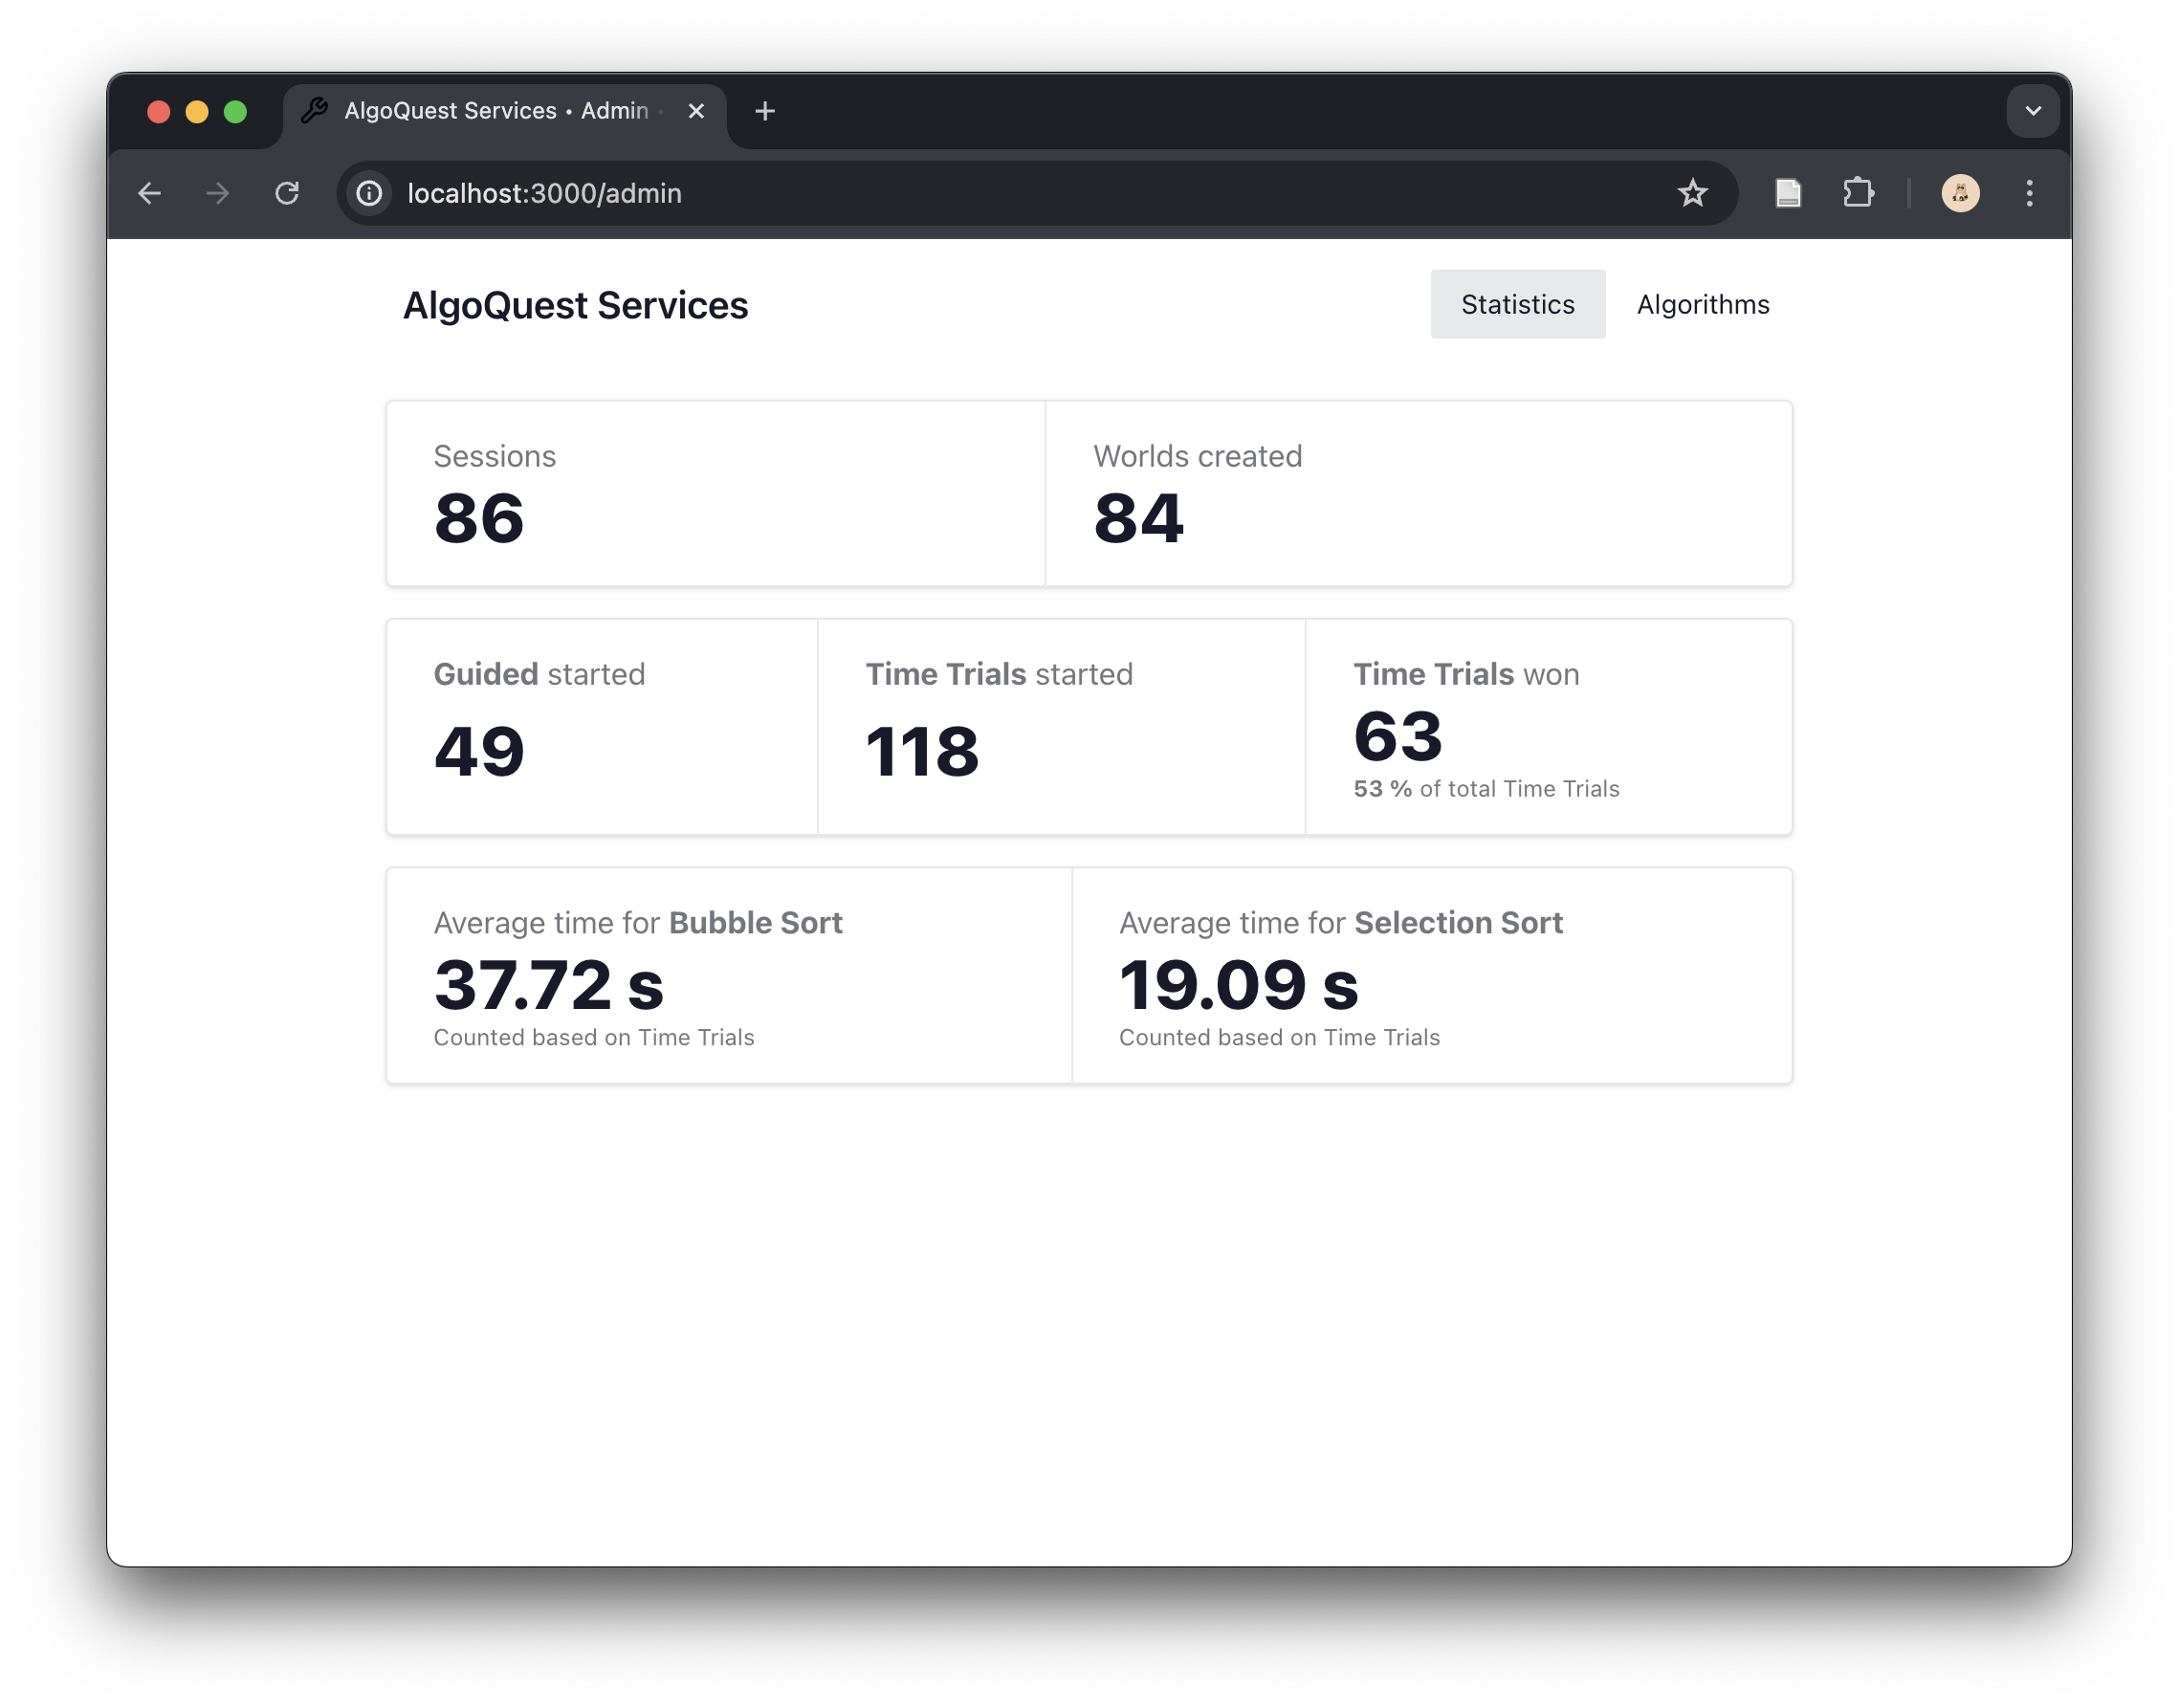
\includegraphics[width=0.7\linewidth]{sections/5/2/images/admin_dashboard_statistics}
    \caption{Στατιστικά διαχειριστικού}
    \label{fig:admin_dashboard_statistics_results}
\end{figure}

Αξιοσημείωτη είναι η σύγκριση των μέσων χρόνων ολοκλήρωσης των αλγορίθμων. Συγκεκριμένα, οι παίκτες παίρνουν περισσότερο χρόνο για να ολοκληρώσουν τον αλγόριθμο Bubble Sort, κάτι που είναι λογικό, καθώς αυτός ο αλγόριθμος απαιτεί περισσότερα βήματα κατά μέσο όρο σε σχέση με άλλους αλγόριθμους, όπως ο Selection Sort. Αυτό το εύρημα υπογραμμίζει τη σχετική πολυπλοκότητα του Bubble Sort και την ανάγκη των συμμετεχόντων  για περισσότερο χρόνο και εξάσκηση για την κατανόησή του.

Η μεγαλύτερη διάρκεια ολοκλήρωσης για τον Bubble Sort υποδεικνύει επίσης ότι οι μαθητές μπορεί να χρειάζονται επιπλέον εξηγήσεις και πρακτική για να κατανοήσουν τη διαδικασία και τη λογική πίσω από αυτόν τον αλγόριθμο. Οι εκπαιδευτικοί μπορούν να χρησιμοποιήσουν αυτά τα δεδομένα για να εντοπίσουν τα σημεία όπου οι μαθητές δυσκολεύονται περισσότερο και να παρέχουν επιπλέον υποστήριξη και πόρους για την ενίσχυση της κατανόησης.

Η ανάλυση των δεδομένων χρήσης της πλατφόρμας αποκαλύπτει επίσης τη συμπεριφορά των μαθητών κατά τη διάρκεια του παιχνιδιού. Για παράδειγμα, το γεγονός ότι περίπου το 50 \% των επιπέδων Time Trial είναι επιτυχή (63 επιτυχίες έναντι 118 προσπαθειών) υποδεικνύει ότι ενώ οι μαθητές βρίσκουν την πρόκληση ελκυστική, υπάρχει επίσης σημαντικός αριθμός αποτυχιών, που μπορεί να οφείλονται σε δυσκολίες στην εφαρμογή των αλγορίθμων υπό χρονική πίεση. Αυτό μπορεί να είναι ένδειξη ότι οι μαθητές χρειάζονται περισσότερη προετοιμασία ή ότι οι εκπαιδευτικοί πρέπει να προσαρμόσουν το επίπεδο δυσκολίας ώστε να ταιριάζει καλύτερα στις ικανότητες των μαθητών τους.

Επιπλέον, η διαφορά στους χρόνους ολοκλήρωσης ανάμεσα στους αλγόριθμους υποδεικνύει την ανάγκη για διαφοροποιημένες εκπαιδευτικές προσεγγίσεις. Ενώ ο αλγόριθμος Bubble Sort απαιτεί περισσότερο χρόνο και ενδεχομένως προκαλεί μεγαλύτερες δυσκολίες, ο αλγόριθμος Selection Sort φαίνεται να είναι πιο προσιτός και κατανοητός από τους μαθητές. Αυτό μπορεί να βοηθήσει τους εκπαιδευτικούς να καθορίσουν ποιοι αλγόριθμοι πρέπει να διδαχθούν πρώτα και πώς να δομηθεί το πρόγραμμα διδασκαλίας για να βελτιωθεί η κατανόηση και η ικανότητα εφαρμογής των μαθητών.

Συνολικά, αυτή η ανάλυση βοηθά τους εκπαιδευτικούς να κατανοήσουν καλύτερα τη χρήση της πλατφόρμας και τις επιδόσεις των μαθητών, επιτρέποντάς τους να προσαρμόσουν κατάλληλα την εκπαιδευτική διαδικασία. Με τη βοήθεια των δεδομένων, μπορούν να βελτιώσουν την εμπειρία μάθησης, να ενισχύσουν τις αδύναμες περιοχές και να προωθήσουν μια πιο αποδοτική και ευχάριστη εκπαίδευση.
